% Options for packages loaded elsewhere
\PassOptionsToPackage{unicode}{hyperref}
\PassOptionsToPackage{hyphens}{url}
%
\documentclass[
  ignorenonframetext,
]{beamer}
\usepackage{pgfpages}
\setbeamertemplate{caption}[numbered]
\setbeamertemplate{caption label separator}{: }
\setbeamercolor{caption name}{fg=normal text.fg}
\beamertemplatenavigationsymbolsempty
% Prevent slide breaks in the middle of a paragraph
\widowpenalties 1 10000
\raggedbottom
\setbeamertemplate{part page}{
  \centering
  \begin{beamercolorbox}[sep=16pt,center]{part title}
    \usebeamerfont{part title}\insertpart\par
  \end{beamercolorbox}
}
\setbeamertemplate{section page}{
  \centering
  \begin{beamercolorbox}[sep=12pt,center]{part title}
    \usebeamerfont{section title}\insertsection\par
  \end{beamercolorbox}
}
\setbeamertemplate{subsection page}{
  \centering
  \begin{beamercolorbox}[sep=8pt,center]{part title}
    \usebeamerfont{subsection title}\insertsubsection\par
  \end{beamercolorbox}
}
\AtBeginPart{
  \frame{\partpage}
}
\AtBeginSection{
  \ifbibliography
  \else
    \frame{\sectionpage}
  \fi
}
\AtBeginSubsection{
  \frame{\subsectionpage}
}

\usepackage{amsmath,amssymb}
\usepackage{lmodern}
\usepackage{iftex}
\ifPDFTeX
  \usepackage[T1]{fontenc}
  \usepackage[utf8]{inputenc}
  \usepackage{textcomp} % provide euro and other symbols
\else % if luatex or xetex
  \usepackage{unicode-math}
  \defaultfontfeatures{Scale=MatchLowercase}
  \defaultfontfeatures[\rmfamily]{Ligatures=TeX,Scale=1}
\fi
% Use upquote if available, for straight quotes in verbatim environments
\IfFileExists{upquote.sty}{\usepackage{upquote}}{}
\IfFileExists{microtype.sty}{% use microtype if available
  \usepackage[]{microtype}
  \UseMicrotypeSet[protrusion]{basicmath} % disable protrusion for tt fonts
}{}
\makeatletter
\@ifundefined{KOMAClassName}{% if non-KOMA class
  \IfFileExists{parskip.sty}{%
    \usepackage{parskip}
  }{% else
    \setlength{\parindent}{0pt}
    \setlength{\parskip}{6pt plus 2pt minus 1pt}}
}{% if KOMA class
  \KOMAoptions{parskip=half}}
\makeatother
\usepackage{xcolor}
\newif\ifbibliography
\usepackage[normalem]{ulem}
\setlength{\emergencystretch}{3em} % prevent overfull lines
\setcounter{secnumdepth}{-\maxdimen} % remove section numbering


\providecommand{\tightlist}{%
  \setlength{\itemsep}{0pt}\setlength{\parskip}{0pt}}\usepackage{longtable,booktabs,array}
\usepackage{calc} % for calculating minipage widths
\usepackage{caption}
% Make caption package work with longtable
\makeatletter
\def\fnum@table{\tablename~\thetable}
\makeatother
\usepackage{graphicx}
\makeatletter
\def\maxwidth{\ifdim\Gin@nat@width>\linewidth\linewidth\else\Gin@nat@width\fi}
\def\maxheight{\ifdim\Gin@nat@height>\textheight\textheight\else\Gin@nat@height\fi}
\makeatother
% Scale images if necessary, so that they will not overflow the page
% margins by default, and it is still possible to overwrite the defaults
% using explicit options in \includegraphics[width, height, ...]{}
\setkeys{Gin}{width=\maxwidth,height=\maxheight,keepaspectratio}
% Set default figure placement to htbp
\makeatletter
\def\fps@figure{htbp}
\makeatother

\makeatletter
\@ifpackageloaded{tcolorbox}{}{\usepackage[many]{tcolorbox}}
\@ifpackageloaded{fontawesome5}{}{\usepackage{fontawesome5}}
\definecolor{quarto-callout-color}{HTML}{909090}
\definecolor{quarto-callout-note-color}{HTML}{0758E5}
\definecolor{quarto-callout-important-color}{HTML}{CC1914}
\definecolor{quarto-callout-warning-color}{HTML}{EB9113}
\definecolor{quarto-callout-tip-color}{HTML}{00A047}
\definecolor{quarto-callout-caution-color}{HTML}{FC5300}
\definecolor{quarto-callout-color-frame}{HTML}{acacac}
\definecolor{quarto-callout-note-color-frame}{HTML}{4582ec}
\definecolor{quarto-callout-important-color-frame}{HTML}{d9534f}
\definecolor{quarto-callout-warning-color-frame}{HTML}{f0ad4e}
\definecolor{quarto-callout-tip-color-frame}{HTML}{02b875}
\definecolor{quarto-callout-caution-color-frame}{HTML}{fd7e14}
\makeatother
\makeatletter
\makeatother
\makeatletter
\makeatother
\makeatletter
\@ifpackageloaded{caption}{}{\usepackage{caption}}
\AtBeginDocument{%
\ifdefined\contentsname
  \renewcommand*\contentsname{Table of contents}
\else
  \newcommand\contentsname{Table of contents}
\fi
\ifdefined\listfigurename
  \renewcommand*\listfigurename{List of Figures}
\else
  \newcommand\listfigurename{List of Figures}
\fi
\ifdefined\listtablename
  \renewcommand*\listtablename{List of Tables}
\else
  \newcommand\listtablename{List of Tables}
\fi
\ifdefined\figurename
  \renewcommand*\figurename{Figure}
\else
  \newcommand\figurename{Figure}
\fi
\ifdefined\tablename
  \renewcommand*\tablename{Table}
\else
  \newcommand\tablename{Table}
\fi
}
\@ifpackageloaded{float}{}{\usepackage{float}}
\floatstyle{ruled}
\@ifundefined{c@chapter}{\newfloat{codelisting}{h}{lop}}{\newfloat{codelisting}{h}{lop}[chapter]}
\floatname{codelisting}{Listing}
\newcommand*\listoflistings{\listof{codelisting}{List of Listings}}
\makeatother
\makeatletter
\@ifpackageloaded{caption}{}{\usepackage{caption}}
\@ifpackageloaded{subcaption}{}{\usepackage{subcaption}}
\makeatother
\makeatletter
\@ifpackageloaded{tcolorbox}{}{\usepackage[many]{tcolorbox}}
\makeatother
\makeatletter
\@ifundefined{shadecolor}{\definecolor{shadecolor}{rgb}{.97, .97, .97}}
\makeatother
\makeatletter
\makeatother
\ifLuaTeX
  \usepackage{selnolig}  % disable illegal ligatures
\fi
\IfFileExists{bookmark.sty}{\usepackage{bookmark}}{\usepackage{hyperref}}
\IfFileExists{xurl.sty}{\usepackage{xurl}}{} % add URL line breaks if available
\urlstyle{same} % disable monospaced font for URLs
\hypersetup{
  pdftitle={La Política de las Finanzas Públicas ~Maestría en Finanzas Públicas Provinciales y Municipales ~Universidad Nacional de La Plata (UNLP)},
  hidelinks,
  pdfcreator={LaTeX via pandoc}}

\title{La Política de las Finanzas Públicas ~Maestría en Finanzas
Públicas Provinciales y Municipales ~Universidad Nacional de La Plata
(UNLP)}
\subtitle{Clase 2. En la vida hay que elegir. ¿Cómo eligen las
sociedades?}
\author{\textbf{Sebastián Freille}\\
sfreille@unc.edu.ar\\
FCE-UNC}
\date{}

\begin{document}
\frame{\titlepage}
\ifdefined\Shaded\renewenvironment{Shaded}{\begin{tcolorbox}[borderline west={3pt}{0pt}{shadecolor}, boxrule=0pt, enhanced, sharp corners, breakable, frame hidden, interior hidden]}{\end{tcolorbox}}\fi

\begin{frame}
\begin{quote}
Una mayoría sujeta a las limitaciones constitucionales y que cambie
fácilmente conforme a los cambios de la opinión popular es el verdadero
soberano de un pueblo libre; el que la deseche cae en la anarquía; la
unanimidad es imposible; rechazando el principio de la mayoría, sólo
queda ya el despotismo\ldots{}\\
\textbf{{[}Abraham Lincoln, \emph{Toma de Posesión} (1861){]}}
\end{quote}
\end{frame}

\begin{frame}{\textbf{El problema de (economía política) la política
económica}}
\protect\hypertarget{el-problema-de-economuxeda-poluxedtica-la-poluxedtica-econuxf3mica}{}
\begin{itemize}
\tightlist
\item
  Problema general de política
\item
  Restricciones sobre preferencias individuales
\item
  Violación de restricciones
\end{itemize}

\begin{block}{Introducción}
\protect\hypertarget{introducciuxf3n}{}
\begin{itemize}
\tightlist
\item
  Elección de la política económica importa una decisión colectiva a
  partir de intereses (preferencias) individuales e instituciones
  políticas determinadas
\item
  Decisiones difieren según instituciones políticas --dictadura versus
  democracia \(\longrightarrow\) tanto en el proceso como en los
  resultados
\item
  Existen dos modelos tipicos de democracia --directa y representativa.
  Si bien difieren en muchos aspectos, ambas tienen en el centro del
  proceso decisorio a mecanismos de votacion.
\end{itemize}
\end{block}

\begin{block}{Democracia directa}
\protect\hypertarget{democracia-directa}{}
\begin{itemize}
\tightlist
\item
  Si bien la democracia directa no se usa como mecanismo principal, los
  países tienen herramientas de participación directa:

  \begin{itemize}
  \tightlist
  \item
    Referendum
  \item
    Consulta popular, vinculante y no vinculante
  \item
    Asambleas al aire libre
  \end{itemize}
\item
  Fuentes y bases de datos:

  \begin{itemize}
  \tightlist
  \item
    Base de datos de IDEA \(\longrightarrow\)
    https://www.idea.int/data-tools/data/direct-democracy
  \item
    Swissvotes \(\longrightarrow\) https://swissvotes.ch/page/home
  \end{itemize}
\end{itemize}
\end{block}

\begin{block}{Democracia directa (cont.)}
\protect\hypertarget{democracia-directa-cont.}{}
\begin{figure}

{\centering 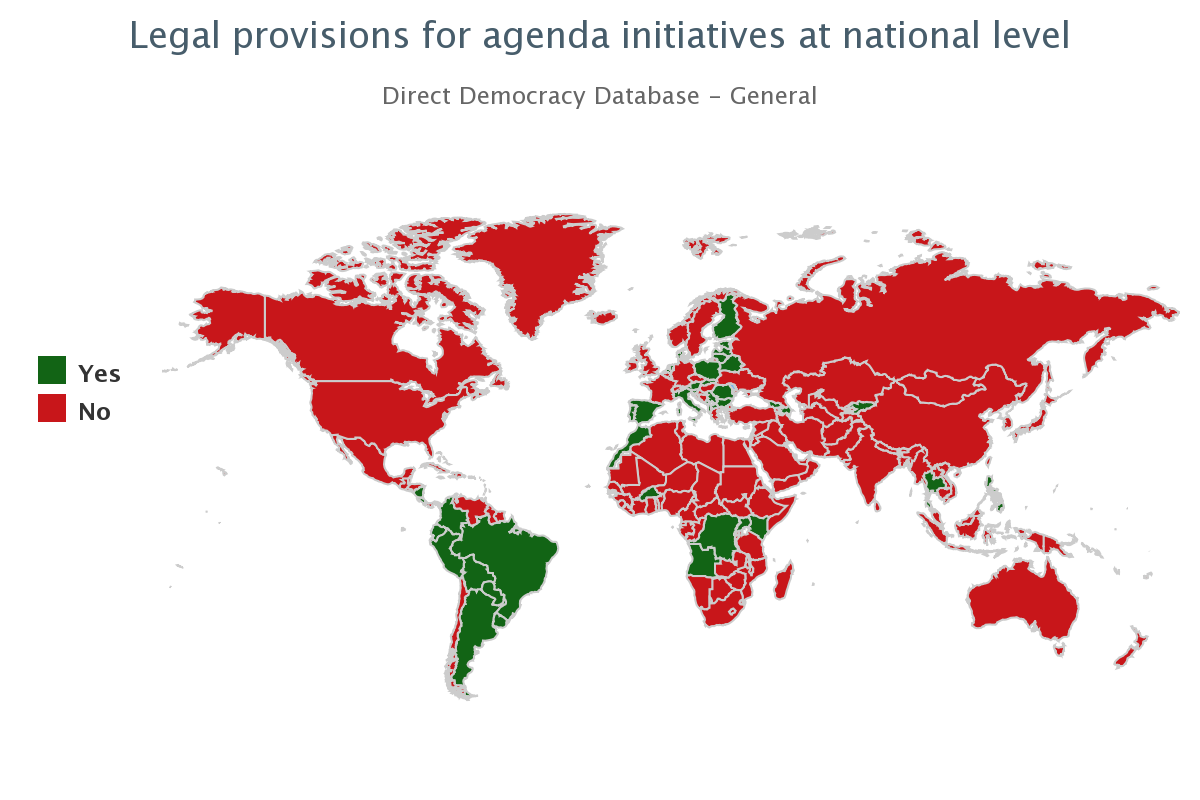
\includegraphics[width=0.9\textwidth,height=\textheight]{../epol/fig/fig-02-010.png}

}

\caption{Provisiones legales para iniciativas de agenda en nivel
nacional}

\end{figure}
\end{block}

\begin{block}{Democracia directa (cont.)}
\protect\hypertarget{democracia-directa-cont.-1}{}
\begin{figure}

{\centering 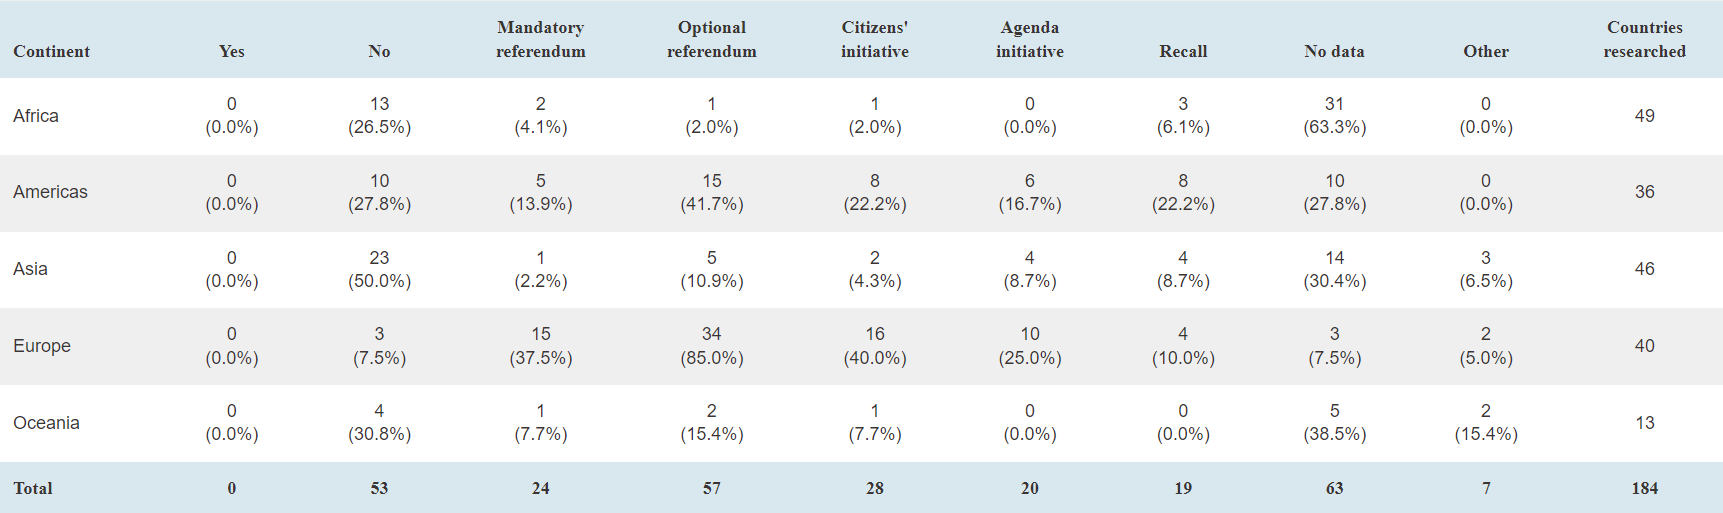
\includegraphics{../epol/fig/fig-02-011.png}

}

\caption{Provisiones legales para democracia directa en nivel local}

\end{figure}
\end{block}

\begin{block}{Problema general de política}
\protect\hypertarget{problema-general-de-poluxedtica}{}
\begin{itemize}
\tightlist
\item
  Un conjuto de ciudadanos --pequeño como en un comité, grande como un
  electorado-afectados por un vector de políticas \textbf{\(q\)}
\item
  Los ciudadanos --\emph{votantes}- están indexados a partir de
  atributos individuales. Entonces, \(\alpha^{i}\) denota las
  características específicas del votante \(i\) (preferencias
  idiosincráticas, dotaciones, riesgos, otros atributos socioeconómicos)
\item
  Los \(\alpha^{i}\)'s se distribuyen entre los individuos de acuerdo a
  una distribución dada
\item
  Los ciudadanos tienen funciones de utilidad sobre canastas de consumo
  \(c^{i}\)
\end{itemize}
\end{block}

\begin{block}{Problema general de política (cont.)}
\protect\hypertarget{problema-general-de-poluxedtica-cont.}{}
\begin{itemize}
\tightlist
\item
  Individuo como \textbf{agente económico} elige su canasta de consumo
  para maximizar su fn. de utilidad sujeto a restricciones
  (presupuestarias/tiempo): \[\begin{aligned}
  U(c^{i},\mathbf{q},\mathbf{p};\alpha^{i}) \\
  H(c^{i},\mathbf{q},\mathbf{p};\alpha^{i}) \geq 0
  \end{aligned}\]
\item
  donde \(\mathbf{p}\) es un vector de variables determinadas en el
  mercado (precios, cantidades). La fn. de utilidad indirecta de \(i\)
  es: \[\begin{aligned}
  \tilde{W}(\mathbf{q},\mathbf{p};\alpha^{i})=\max_{c^{i}}[U(c^{i},\mathbf{q},\mathbf{p};\alpha^{i})\mid H(c^{i},\mathbf{q},\mathbf{p};\alpha^{i})  \geq 0]
  \end{aligned}\]
\end{itemize}
\end{block}

\begin{block}{Problema general de política (cont.)}
\protect\hypertarget{problema-general-de-poluxedtica-cont.-1}{}
\begin{itemize}
\tightlist
\item
  El gobierno como \textbf{policymaker} fija vector de políticas
  \(\mathbf{q}\) bajo ciertas restricciones: respetar los valores de
  \(\mathbf{p}\) dados en el mercado, presupuesto equilibrado, y otras.
  Así: \[\begin{aligned}
  G(\mathbf{q},\mathbf{p})\geq 0
  \end{aligned}\]
\item
  Si las restricciones son vinculantes entonces,
  \(\mathbf{p}=P(\mathbf{q})\) --esto es, los valores de mercado
  dependerán de \(\mathbf{q}\) y de parámetros
\item
  El individuo como \textbf{agente político} actúa como votante,
  lobista, y otras. Sus acciones están determinadas por sus
  \emph{preferencias de política} --obtenidas de su fn. de utilidad
  indirecta, \(\tilde{W}\).
\end{itemize}
\end{block}

\begin{block}{Problema general de política (cont.)}
\protect\hypertarget{problema-general-de-poluxedtica-cont.-2}{}
\begin{itemize}
\tightlist
\item
  Las preferencias de política de forma reducida son: \[\begin{aligned}
  \tilde{W}(\mathbf{q},P(\mathbf{q});\alpha^{i})
  \end{aligned}\]
\item
  La política preferida, o\textbf{punto ideal}, del votante \(i\) es:
  \[\begin{aligned}
  \mathbf{q(\alpha^{i})}=\arg\max_{q} W(\mathbf{q};\alpha^{i})
  \end{aligned}\]
\item
  El \textbf{conflicto en las preferencias de política surge por las
  diferencias en \(\alpha^{i}\)}.
\end{itemize}
\end{block}

\begin{block}{Problema de política con 2 (dos) individuos}
\protect\hypertarget{problema-de-poluxedtica-con-2-dos-individuos}{}
\begin{itemize}
\tightlist
\item
  Individuos maximizan una función de utilidad
  \(U(x_{1},x_{2};\alpha^{i})\) --\(x_{1}\) y \(x_{2}\) bienes privados.
  El gobierno le saca \(\tau\) del \(Y\) al individuo y le devuelve
  \(T\) como transferencia de suma fija
  \[p_{1}x_{1}+p_{2}x_{2} \leq (1-\tau)Y+T\]
\item
  El problema consiste en maximizar la utilidad sujeta a la restricción
  presupuestaria \(\longrightarrow\) se obtienen las demandas
  individuales \(x_{1}(p_{1},p_{2},Y,\tau,T;\alpha^{i})\) y
  \(x_{2}(p_{1},p_{2},Y,\tau,T;\alpha^{i})\)
\item
  El parámetro \(\alpha\) en la función de utilidad captura la
  heterogeneidad de preferencias
\end{itemize}
\end{block}

\begin{block}{Problema de política con 2 (dos) individuos}
\protect\hypertarget{problema-de-poluxedtica-con-2-dos-individuos-1}{}
\begin{itemize}
\tightlist
\item
  Reemplazando demanda en la fn. de utilidad, tenemos la fn. de utilidad
  indirecta: \[\begin{aligned}
            V(p_{1},p_{2},Y,,\tau,T;\alpha^{i}) \equiv \\
            U(x_{1}(p_{1},p_{2},Y,\tau,T;\alpha^{i}),x_{2}(p_{1},p_{2},Y,\tau,T;\alpha^{i});\alpha^{i})
          \end{aligned}\]
\item
  Importante \(\longrightarrow\) utilidad es función de las variables de
  política {[}dado que \(x_{1}\) y \(x_{2}\) son elegidos de manera
  óptima{]} \[\begin{aligned}
    V(\tau,T;\alpha^{i}) \equiv \\ V(p_{1}(\tau,T),p_{2}(\tau,T),Y(\tau,T),\tau,T;\alpha^{i})
              \end{aligned}\]
\end{itemize}
\end{block}

\begin{block}{Problema de política con 2 (dos) individuos}
\protect\hypertarget{problema-de-poluxedtica-con-2-dos-individuos-2}{}
\begin{itemize}
\tightlist
\item
  Conociendo \(\tau\) conocemos \(T\) {[}¿por qué?{]} y la fn. UI:
  \[V(\tau;\alpha^{i})\]
\item
  Política preferida por \emph{i} se obtiene hallando \(\tau\) que
  maximiza U indirecta:
  \[\frac{\partial V(\tau;\alpha^{i})}{\partial \tau}=0\]
\item
  \(\tau^{*}(\alpha^{i})\) \(\longrightarrow\) dimensión política
  evidente --\(\alpha^{i}\)'s diferentes implican políticas (alícuotas)
  preferidas diferentes
\end{itemize}
\end{block}

\begin{block}{Ilustración y aplicación}
\protect\hypertarget{ilustraciuxf3n-y-aplicaciuxf3n}{}
\begin{itemize}
\tightlist
\item
  Evidencia sugiere que no hay diferencias significativas en el apoyo a
  mayor redistribución en EEUU de acuerdo a diferencias etarias, de
  etnia y género. Incluso hay dos grupos que han disminuido su apoyo a
  la redistribución: los adultos mayores y los afroamericanos.
  Sorprendemente son dos de los grupos más dependientes en
  transferencias desde el estado {[}Ashok, V., Kuziemko, I., \&
  Washington, E. (2015){]}.
\item
  Stantcheva (2021) estudia el apoyo a la redistribución usando
  experimentos sociales de gran escala (videos informativos) y estudia
  diferencias según género, etnia, nivel de ingreso e
  ideología/afiliación.
\end{itemize}
\end{block}

\begin{block}{Ilustración y aplicación (cont.).}
\protect\hypertarget{ilustraciuxf3n-y-aplicaciuxf3n-cont..}{}
\begin{figure}

{\centering 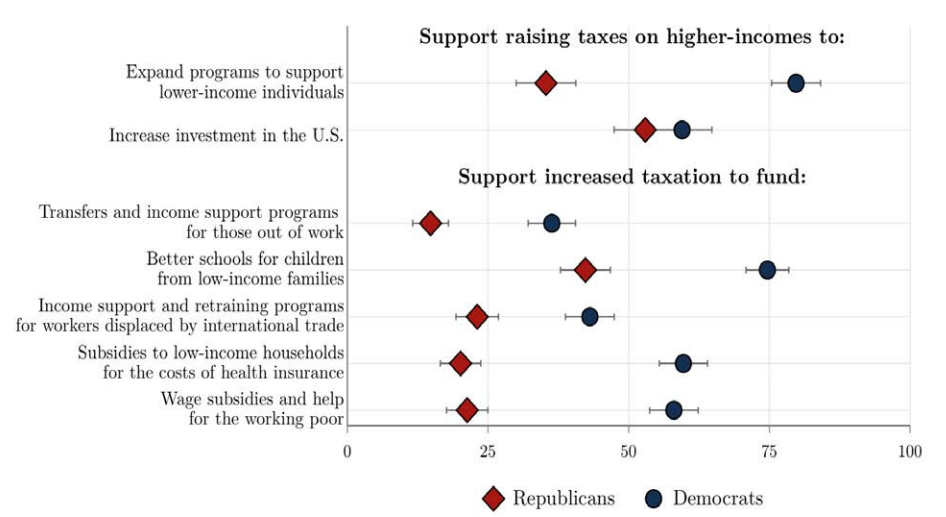
\includegraphics{../epol/fig/fig-02-001.png}

}

\caption{Grado de apoyo a redistribución - Ideología/Partidismo}

\end{figure}
\end{block}

\begin{block}{Ilustración y aplicación (cont.)}
\protect\hypertarget{ilustraciuxf3n-y-aplicaciuxf3n-cont.}{}
\begin{figure}

{\centering 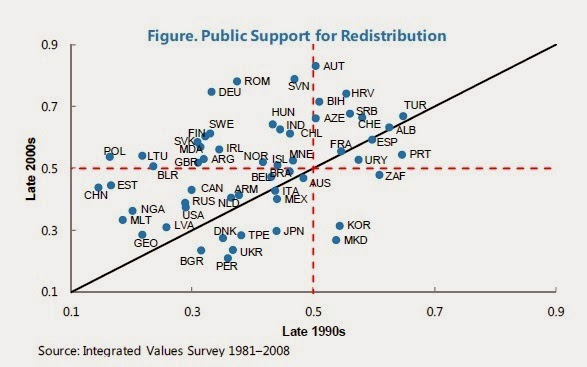
\includegraphics[width=0.9\textwidth,height=\textheight]{../epol/fig/fig-02-002.jpg}

}

\caption{Grado de apoyo a redistribución - Evolución}

\end{figure}
\end{block}

\begin{block}{Ilustración y aplicación (cont.)}
\protect\hypertarget{ilustraciuxf3n-y-aplicaciuxf3n-cont.-1}{}
\begin{figure}

{\centering 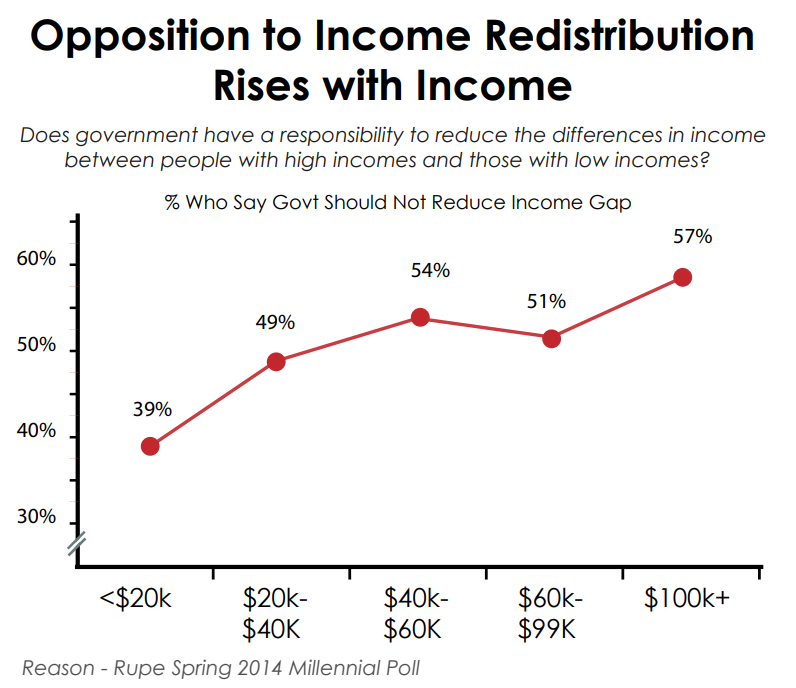
\includegraphics[width=0.7\textwidth,height=\textheight]{../epol/fig/fig-02-003.png}

}

\caption{Grado de apoyo a redistribución de millenials - Edad e
ingresos}

\end{figure}
\end{block}
\end{frame}

\begin{frame}{\textbf{Preferencias y alternativas}}
\protect\hypertarget{preferencias-y-alternativas}{}
\begin{itemize}
\tightlist
\item
  Preferencias y propiedades
\item
  Casos de 2 y más alternativas
\end{itemize}

\begin{block}{Preferencia y elección}
\protect\hypertarget{preferencia-y-elecciuxf3n}{}
\begin{itemize}
\tightlist
\item
  Sea un individuo, \(i\), y 3 objetos --``alternativas''-, \(A\),
  \(B\), y \(C\) sobre los que \(i\) tiene preferencias
\item
  El individuo \(i\) es capaz de evaluar:

  \begin{itemize}
  \tightlist
  \item
    ``Prefiero \(A\) a \(B\)''
  \item
    ``Soy indiferente entre \(B\) y \(C\)''.
  \end{itemize}
\item
  La relación \(A \succ B\) representa al primer enunciado; la relación
  \(B \sim C\) representa al segundo
\item
  La \textbf{elección} de \(i\) es racional si está de acuerdo con su
  \textbf{preferencia}. Sujetas a ciertas propiedades que permita
  ``ordenarlas''
\end{itemize}
\end{block}

\begin{block}{Preferencia y elección (cont.)}
\protect\hypertarget{preferencia-y-elecciuxf3n-cont.}{}
\begin{itemize}
\tightlist
\item
  Sean \(A\) y \(B\) dos alternativas de política. Un individuo vota por
  \(A\) siempre que \(W(A) \geq W(B)\).
\item
  Sea \(\succeq_{i}\) una relacion binaria tal que \(A \succ_{i} B\)
  significa que el individuo \emph{i} prefiere a \(A\)
  --\(W(A) \geq W(B)\) y donde \(\succeq_{i}\) cumple con las
  propiedades estándares de las preferencias

  \begin{itemize}
  \tightlist
  \item
    \textbf{Completas:} \(A \preceq_{i} B\), o \(B \preceq_{i} A\), o
    ambas -- en este caso el individuo es indiferente
  \item
    \textbf{Transitivas:} si \(B \preceq_{i} A\) y \(A \preceq_{i} C\),
    entonces \(C \preceq_{i} A\)
  \end{itemize}
\item
  Como puede verse las preferencias están dadas al nivel individual
\end{itemize}
\end{block}

\begin{block}{Ordenamiento de preferencias}
\protect\hypertarget{ordenamiento-de-preferencias}{}
\begin{itemize}
\tightlist
\item
  Si las preferencias de \(i\) satisfacen estas propiedades, decimos que
  \(i\) tiene un \textbf{ordenamiento de preferencias racional}. La
  elección racional será la que esté al inicio (izquierda) del
  ordenamiento
\item
  No todas las relaciones entre ``alternativas'' son \textbf{completas}
  o \textbf{transitivas}. Ejemplos:

  \begin{itemize}
  \tightlist
  \item
    La comparación debe tener sentido \(\longrightarrow\) elegir entre
    cosas desconocidas (comparabilidad)
  \item
    La comparación debe ser sobre algo que le importa al individuo
  \end{itemize}
\end{itemize}
\end{block}

\begin{block}{Caso: Dos alternativas}
\protect\hypertarget{caso-dos-alternativas}{}
\begin{itemize}
\tightlist
\item
  Condiciones deseadas de un sistema de reglas de votación entre dos
  alternativas:

  \begin{itemize}
  \tightlist
  \item
    \textbf{Anonimidad} \(\longrightarrow\) si 2 votantes intercambian
    sus votos antes de emitirlos, el resultado de la elección no cambia
    (votantes simétricos)
  \item
    \textbf{Neutralidad} \(\longrightarrow\) si cada votante revierte su
    orden de preferencia --i.e si votó A, ahora vota B y viceversa-, el
    resultado de la elección se revierte (alternativas simétricas)
  \item
    \textbf{Monotonicidad} \(\longrightarrow\) si un votante único que
    originalmente votó por el perdedor elección, ahora vota por el
    ganador, el ganador de la elección sigue siendo el mismo.
  \end{itemize}
\end{itemize}
\end{block}

\begin{block}{Caso: Dos alternativas (cont.)}
\protect\hypertarget{caso-dos-alternativas-cont.}{}
\begin{itemize}
\tightlist
\item
  Siempre que el número de votantes sea impar, habrá un resultado
  cierto. Si se vota por regla de mayoría absoluta, se elegirá la opción
  preferida por una mayoría de votantes, i.e.~\(\frac{N+1}{2}\)
\end{itemize}

\begin{tcolorbox}[enhanced jigsaw, titlerule=0mm, breakable, colback=white, left=2mm, coltitle=black, toptitle=1mm, leftrule=.75mm, opacityback=0, bottomtitle=1mm, opacitybacktitle=0.6, colbacktitle=quarto-callout-important-color!10!white, title={Teorema de May}, toprule=.15mm, colframe=quarto-callout-important-color-frame, rightrule=.15mm, arc=.35mm, bottomrule=.15mm]

El único método que satisface las condiciones de anonimidad, neutralidad
y monotonicidad para determinar un ganador de una elección entre dos
alternativas es la regla de la mayoría absoluta.

\end{tcolorbox}
\end{block}

\begin{block}{Caso: Dos alternativas (cont.)}
\protect\hypertarget{caso-dos-alternativas-cont.-1}{}
\begin{itemize}
\tightlist
\item
  \(A \succ_{1} B\)
\item
  \(A \succ_{2} B\)
\item
  \(B \succ_{3} A\)
\end{itemize}

\begin{quote}
El ganador es \(A\). ¿Que pasa si intercambian sus votos? (anonimidad)
\end{quote}

\begin{itemize}
\tightlist
\item
  \(A \succ_{1} B\)
\item
  \(B \succ_{3} A\)
\item
  \(A \succ_{2} B\)
\end{itemize}
\end{block}
\end{frame}

\begin{frame}
\begin{quote}
¿Que pasa si cada uno revierte su preferencia? (neutralidad)
\end{quote}

\begin{itemize}
\tightlist
\item
  \(B \succ_{1} A\)
\item
  \(B \succ_{2}A\)
\item
  \(A \succ_{3} B\)
\end{itemize}

\begin{quote}
Qué pasa si votó antes por el perdedor, ahora vota por el ganador?
(monotonicidad)
\end{quote}

\begin{itemize}
\tightlist
\item
  \(A \succ_{1} B\)
\item
  \(A \succ_{2} B\)
\item
  \(A \succ_{3} B\)
\end{itemize}

\begin{block}{Caso: 3 o más alternativas}
\protect\hypertarget{caso-3-o-muxe1s-alternativas}{}
\begin{itemize}
\tightlist
\item
  ¿Qué sucede si, como en situaciones de la vida real hay más de 2
  alternativas?
\item
  El problema se vuelve más complejo. Problema \(\longrightarrow\)
  existe alguna regla de votación que permita agregar preferencias
  individuales en preferencias sociales y que produzca un claro ganador
  y que satisfaga propiedades deseadas?

  \begin{itemize}
  \tightlist
  \item
    La respuesta es \textbf{no}.
  \end{itemize}
\end{itemize}
\end{block}

\begin{block}{Caso: 3 o más alternativas (cont.)}
\protect\hypertarget{caso-3-o-muxe1s-alternativas-cont.}{}
\hypertarget{tab:tab1}{}
\begin{longtable}[]{@{}cccc@{}}
\toprule()
Orden & Juan & Pedro & María \\
\midrule()
\endhead
1 & A & C & B \\
2 & B & A & C \\
3 & C & B & A \\
\bottomrule()
\end{longtable}

\begin{itemize}
\tightlist
\item
  ¿Hay ganador por mayoría absoluta? No.~Ninguna tiene la mitad mas uno
  de los votos (2). ¿Hay ganador por mayoría simple (pluralidad)?
  No.~Ninguna alternativa tiene más votos que otra --ie. hay triple
  empate.
\end{itemize}
\end{block}

\begin{block}{Caso: 3 o más alternativas (cont.)}
\protect\hypertarget{caso-3-o-muxe1s-alternativas-cont.-1}{}
\begin{tcolorbox}[enhanced jigsaw, titlerule=0mm, breakable, colback=white, left=2mm, coltitle=black, toptitle=1mm, leftrule=.75mm, opacityback=0, bottomtitle=1mm, opacitybacktitle=0.6, colbacktitle=quarto-callout-important-color!10!white, title={Teorema de la imposibilidad de Arrow}, toprule=.15mm, colframe=quarto-callout-important-color-frame, rightrule=.15mm, arc=.35mm, bottomrule=.15mm]

No existe una función de ordenamiento social \(\succ\) tal que para
cualquier grupo G cuyos miembros tengan todos preferencias racionales,
\(\succ\) sea un ordenamiento racional (transitivo) y que satisfaga los
cuatros supuestos de dominio universal, optimalidad de Pareto,
independencia de alternativas irrelevantes y no dictadura.

\end{tcolorbox}

\begin{itemize}
\tightlist
\item
  Si queremos una función de ordenamiento social que cumpla con todas
  esas propiedades, no será transitiva \(\longrightarrow\) habrá ciclos.
\end{itemize}
\end{block}
\end{frame}

\begin{frame}{\textbf{Resolviendo el problema}}
\protect\hypertarget{resolviendo-el-problema}{}
\begin{itemize}
\tightlist
\item
  El teorema de la imposibilidad
\item
  Restringiendo preferencias e instituciones
\item
  Políticas unidimensionales vs multidimensionales
\item
  Aplicación: Redistribución con imposición
\end{itemize}

\begin{block}{Resolviendo el problema}
\protect\hypertarget{resolviendo-el-problema-1}{}
\begin{quote}
Un tratamiento positivo del problema general de política económica
involucra especificar un diseño institucional específico y preguntarse
como el mismo agrega las acciones políticas, basadas en las preferencias
de política individuales, en políticas de equilibrio.
\end{quote}

\ldots{} pero \ldots{}
\end{block}

\begin{block}{Pasaron cosas\ldots{}}
\protect\hypertarget{pasaron-cosas}{}
\begin{figure}

{\centering 
\includegraphics{../epol/fig/fig-02-004.jpg}

}

\caption{El Teorema de la Imposibilidad dice que no}

\end{figure}
\end{block}

\begin{block}{Restricciones y supuestos}
\protect\hypertarget{restricciones-y-supuestos}{}
\begin{itemize}
\tightlist
\item
  Aún la \textbf{regla de mayoría} utilizada extensivamente en
  elecciones alrededor del mundo no es suficiente para producir
  políticas de equilibrio bien definidas
\item
  Para producir estas políticas de equilibrio bien definidas, se deben
  suponer/restringir una de dos cosas:

  \begin{enumerate}
  \tightlist
  \item
    Las preferencias de política individuales a ciertas formas
  \item
    Las instituciones políticas a ciertos tipos
  \end{enumerate}
\end{itemize}
\end{block}

\begin{block}{Agregación de preferencias}
\protect\hypertarget{agregaciuxf3n-de-preferencias}{}
\begin{itemize}
\tightlist
\item
  Agregación de preferencias bajo \textbf{regla de mayoría pura},
  definida como:

  \begin{enumerate}
  \tightlist
  \item
    \textbf{Democracia directa} \(\longrightarrow\) los ciudadanos
    eligen \emph{directamente} las alternativas
  \item
    \textbf{Voto sincero} \(\longrightarrow\) en toda votación, cada
    ciudadano \emph{vota} por la alternativa que le da la mayor utilidad
    de acuerdo a sus preferencias de política (fn. de utilidad
    indirecta), \(W(\mathbf{q};\alpha^{i})\).
  \item
    \textbf{Agenda abierta} \(\longrightarrow\) cada ciudadano vota
    entre pares de alternativas en sucesivas rondas --votación Condorcet
    (\emph{pairwise voting}, en inglés)
  \end{enumerate}
\end{itemize}
\end{block}

\begin{block}{Políticas unidimensionales}
\protect\hypertarget{poluxedticas-unidimensionales}{}
\begin{tcolorbox}[enhanced jigsaw, titlerule=0mm, breakable, colback=white, left=2mm, coltitle=black, toptitle=1mm, leftrule=.75mm, opacityback=0, bottomtitle=1mm, opacitybacktitle=0.6, colbacktitle=quarto-callout-note-color!10!white, title={Definición 1}, toprule=.15mm, colframe=quarto-callout-note-color-frame, rightrule=.15mm, arc=.35mm, bottomrule=.15mm]

Un \textbf{ganador de Condorcet} es una política \(\mathbf{q^{*}}\) tal
que vence a cualquier otra política factible en una votación de a pares

\end{tcolorbox}

\begin{itemize}
\tightlist
\item
  Sea un espacio de política unidimensional de modo que \(q\) es un
  escalar. Según Black (1948), las preferencias de políticas
  \[\begin{aligned}
  \mathbf{q(\alpha^{i})}=\arg\max_{q} W(\mathbf{q};\alpha^{i})
  \end{aligned}\]
\item
  son de \emph{pico único} para \(i\) si su ord. de pref. se rige por la
  distancia a su punto ideal, \(q(\alpha^{i})\): una política más
  cercana a \(q(\alpha^{i})\) es preferida a una(s) mas lejana(s).
\end{itemize}
\end{block}
\end{frame}

\begin{frame}
\begin{block}{Políticas unidimensionales (cont.)}
\protect\hypertarget{poluxedticas-unidimensionales-cont.}{}
\begin{quote}
\textbf{Marie-Jean-Antoine-Nicolas de Caritat, marquis de Condorcet.}
Filósofo y matemático francés. Fue un precursor de los derechos humanos,
el reclamo de justicia, las ideas democráticas y de los derechos de las
mujeres. Durante su vida combinó el pensamiento analítico y formal con
sus acciones e ideas políticas --pasó de apoyar una monarquía
constitucional a una república democrática y de apoyar el voto
calificado (según bienes) al voto uniersal. Murió en la cárcel luego de
huir durante años de las autoridades de la Revolución Francesa. Dejó dos
ideas memorables para la ciencia y economía política: 1) la paradoja de
Condorcet; 2) el teorema del jurado.
\end{quote}
\end{block}

\begin{block}{Políticas unidimensionales (cont.).}
\protect\hypertarget{poluxedticas-unidimensionales-cont..}{}
\begin{tcolorbox}[enhanced jigsaw, titlerule=0mm, breakable, colback=white, left=2mm, coltitle=black, toptitle=1mm, leftrule=.75mm, opacityback=0, bottomtitle=1mm, opacitybacktitle=0.6, colbacktitle=quarto-callout-important-color!10!white, title={El teorema del jurado}, toprule=.15mm, colframe=quarto-callout-important-color-frame, rightrule=.15mm, arc=.35mm, bottomrule=.15mm]

Dado un grupo de votantes (``un jurado'') decidiendo independientemente
entre un resultado correcto con \emph{\(prob\)} \(0 \leq 1\) y un
resultado incorrecto con \emph{\(prob\)} \(1-p\). 1. Si \(p > 1/2\)
(c/votante tiende a votar más correcto que incorrecto), añadir más
votantes aumenta la \emph{\(prob\)} de que la mayoría elija
correctamente y la \emph{\(prob\)} de una decisión correcta tiende a 1
2. Si \(p < 1/2\) (c/votante tiende a votar más incorrecto que
correcto), añadir más votantes disminuye la \emph{\(prob\)} de que la
mayoría elija correctamente y la \emph{\(prob\)} de una decisión
correcta se maximiza para un tamaño igual a 1.

\end{tcolorbox}

\begin{itemize}
\tightlist
\item
  Link: \href{https://www.geogebra.org/m/ntctceas}{Teorema del jurado}
\end{itemize}
\end{block}

\begin{block}{Preferencias de pico único}
\protect\hypertarget{preferencias-de-pico-uxfanico}{}
\begin{tcolorbox}[enhanced jigsaw, titlerule=0mm, breakable, colback=white, left=2mm, coltitle=black, toptitle=1mm, leftrule=.75mm, opacityback=0, bottomtitle=1mm, opacitybacktitle=0.6, colbacktitle=quarto-callout-note-color!10!white, title={Definición 2}, toprule=.15mm, colframe=quarto-callout-note-color-frame, rightrule=.15mm, arc=.35mm, bottomrule=.15mm]

Las preferencias de política del votante \(i\) son \textbf{de pico
único} si lo siguiente se cumple:\\
Si \(q^{''} \leq q^{'} \leq q(\alpha^{i})\) o
\(q^{''} \geq q^{'} \geq q(\alpha^{i})\), entonces\\
\(W(q^{''};\alpha^{i}) \leq W(q^{'};\alpha^{i})\)

\end{tcolorbox}

\begin{itemize}
\tightlist
\item
  Un primer resultado simple pero útil es:
\end{itemize}

\begin{tcolorbox}[enhanced jigsaw, titlerule=0mm, breakable, colback=white, left=2mm, coltitle=black, toptitle=1mm, leftrule=.75mm, opacityback=0, bottomtitle=1mm, opacitybacktitle=0.6, colbacktitle=quarto-callout-tip-color!10!white, title={Proposición 1}, toprule=.15mm, colframe=quarto-callout-tip-color-frame, rightrule=.15mm, arc=.35mm, bottomrule=.15mm]

Si todos los votantes tienen preferencias de política de pico único
sobre un ordenamiento dado de alternativas de política, un ganador de
Condorcet siempre existe y coincide con el punto ideal del mediano

\end{tcolorbox}
\end{block}

\begin{block}{Preferencias de pico único (cont.)}
\protect\hypertarget{preferencias-de-pico-uxfanico-cont.}{}
\begin{itemize}
\tightlist
\item
  Considere 3 (tres) individuos que difieren sólo en sus niveles de
  ingreso (y eso moldea sus prefs. por políticas). El individuo 1 es de
  \(Y\) alto (prefiere \(T\) bajos), el individuo 2 es de \(Y\) medio y
  prefiere \(T\) medianos y el individuo 3 es de \(Y\) bajo y prefiere
  \(T\) altos.
\item
  Si \(A\), \(B\) y \(C\) son tasas bajas, medias y altas
  respectivamente entonces: \[\begin{aligned}
  \tau^{*}(\alpha^{1})=A \\
  \tau^{*}(\alpha^{2})=B \\
  \tau^{*}(\alpha^{3})=C \\
  \end{aligned}\]
\item
  En base a la figura, exprese el orden de preferencias de cada
  individuo. ¿Qué nota?
\end{itemize}
\end{block}

\begin{block}{Preferencias de pico único (cont.)}
\protect\hypertarget{preferencias-de-pico-uxfanico-cont.-1}{}
\begin{figure}

{\centering 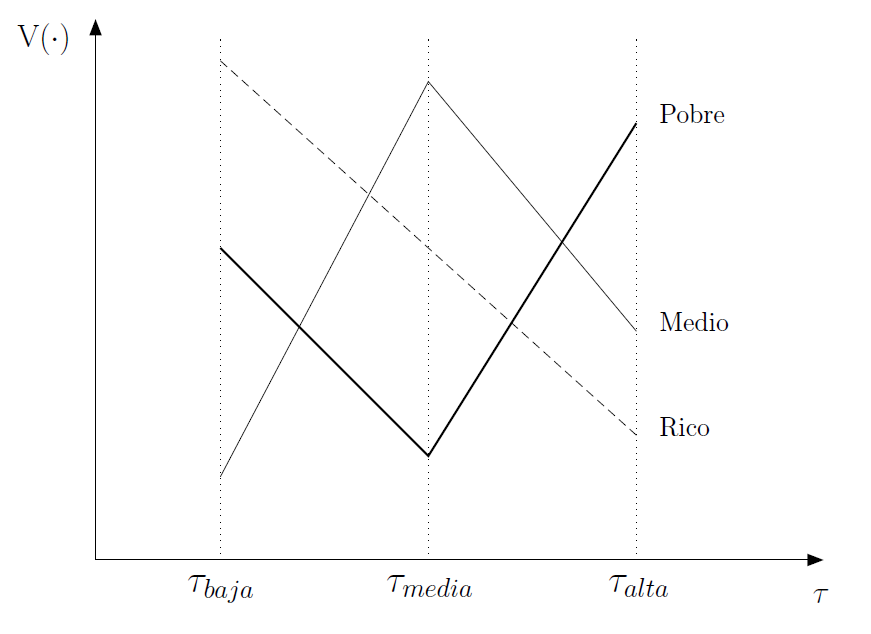
\includegraphics[width=0.8\textwidth,height=\textheight]{../epol/fig/fig-02-013.png}

}

\caption{Preferencias de política (\(\tau\)) {[}Fuente: Fergusson y
Querubin (2018){]}}

\end{figure}
\end{block}

\begin{block}{Políticas unidimensionales (cont.)}
\protect\hypertarget{poluxedticas-unidimensionales-cont.-1}{}
\emph{Fijamos el vector de parámetros a un valor dado, ordenamos a los
individuos en función de sus puntos ideales \(q(\alpha^{i})\) y
etiquetamos al punto ideal del mediano como \(q^{m}\). Suponga que
\(q^{m}\) se enfrenta en votación de a pares a cualquier otra política
\(q^{''}<q^{m}\). De acuerdo a la Definición 2, cualquier individuo cuyo
punto ideal satisface \(q^{m} \leq q(\alpha^{i})\) prefiere \(q^{m}\) a
\(q^{''}\) dado que está más cerca de su punto ideal. Por el supuesto de
voto sincero (A2), votan por \(q^{m}\). La coalición que vota por
\(q^{m}\) entonces constituye una mayoría. Por razonamiento análogo a
\(q^{''}>q^{m}\), obtenemos el resultado de que \(q^{m}\) es un ganador
de Condorcet}
\end{block}

\begin{block}{El votante mediano}
\protect\hypertarget{el-votante-mediano}{}
\begin{tcolorbox}[enhanced jigsaw, titlerule=0mm, breakable, colback=white, left=2mm, coltitle=black, toptitle=1mm, leftrule=.75mm, opacityback=0, bottomtitle=1mm, opacitybacktitle=0.6, colbacktitle=quarto-callout-tip-color!10!white, title={Corolario 1}, toprule=.15mm, colframe=quarto-callout-tip-color-frame, rightrule=.15mm, arc=.35mm, bottomrule=.15mm]

\(q^{m}\) es la única política de equilibrio (punto estable) bajo regla
de mayoría pura, esto es bajo supuestos A1-A3.

\end{tcolorbox}

\begin{itemize}
\tightlist
\item
  La intuición es sencilla: \(q^{m}\) vence a cualquier otro ganador
  previo apenas se presenta y no puede luego ser vencida en ninguna
  votación de a pares sucesiva
\item
  Hay dos supuestos bastante fuertes detrás de este resultado: 1)
  unidimensionalidad; 2) preferencias de pico único.
\end{itemize}
\end{block}

\begin{block}{El votante mediano (cont.)}
\protect\hypertarget{el-votante-mediano-cont.}{}
\begin{figure}

{\centering 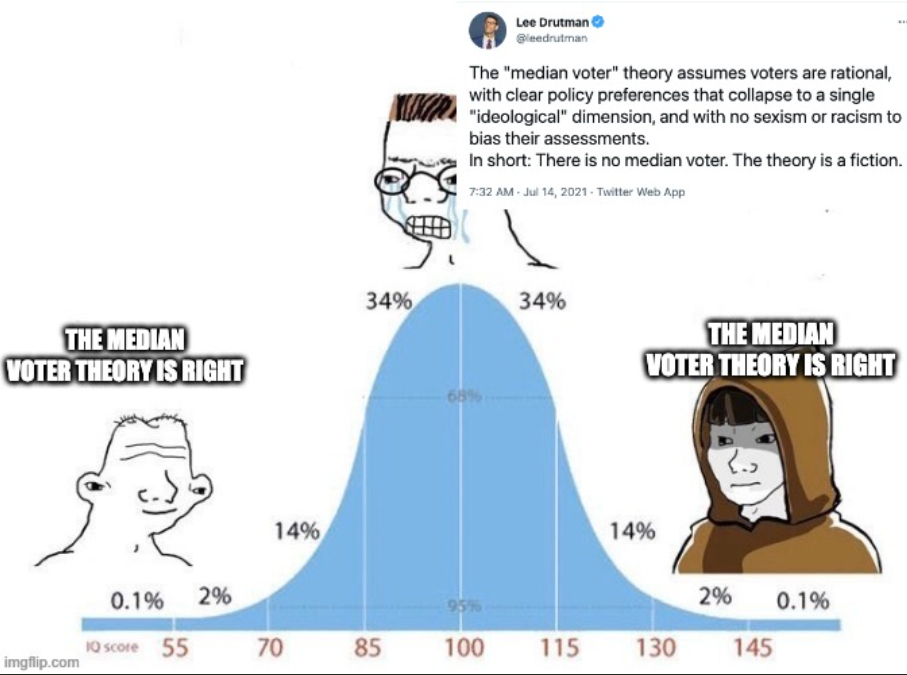
\includegraphics{../epol/fig/fig-02-mvt-meme.png}

}

\caption{El votante mediano no existe!}

\end{figure}
\end{block}

\begin{block}{Aplicación: Preferencias s/aborto}
\protect\hypertarget{aplicaciuxf3n-preferencias-saborto}{}
\begin{itemize}
\tightlist
\item
  Cuestión del aborto en EEUU \(\longrightarrow\) polarización

  \begin{itemize}
  \tightlist
  \item
    Provida (V) \(\longrightarrow\) prohibir aborto totalmente;
    Proeleccion (E) \(\longrightarrow\) derecho absoluto a elegir;
    Roe-Wade (R) \(\longrightarrow\) aborto en etapa temprana. ¿Cuáles
    son las preferencias?

    \begin{itemize}
    \tightlist
    \item
      \(V \succ_{v} R \succ_{v} E\) (provida)
    \item
      \(E \succ_{e} R \succ_{e} V\) (proeleccion)
    \item
      \(R \succ_{rw1} V \succ_{rw1} E\) (roe-wade1)
    \item
      \(R \succ_{rw2} E \succ_{rw2} V\) (roe-wade2)
    \end{itemize}
  \end{itemize}
\item
  Ninguno de los grupos considera a \(R\) como la peor alternativa
  \(\longrightarrow\) ¿consenso?
\end{itemize}
\end{block}

\begin{block}{Aplicación: Preferencias s/aborto (cont.)}
\protect\hypertarget{aplicaciuxf3n-preferencias-saborto-cont.}{}
\begin{figure}

{\centering 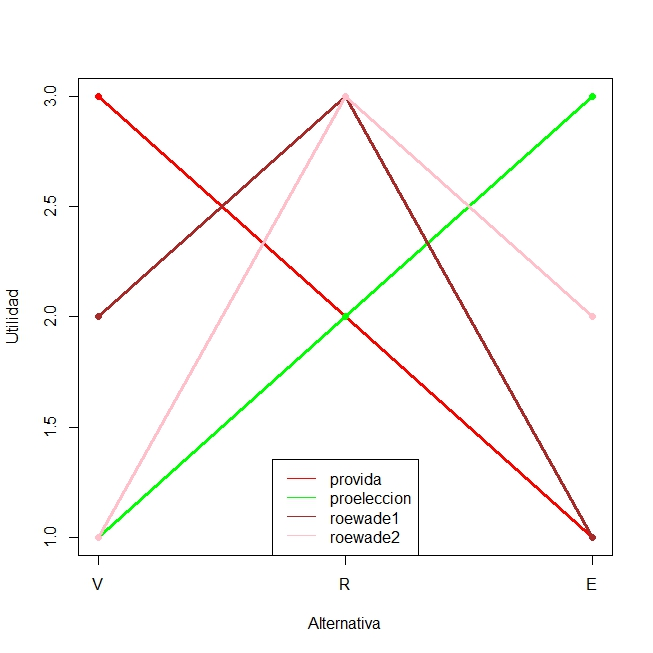
\includegraphics[width=0.7\textwidth,height=\textheight]{../epol/fig/fig-02-012.jpeg}

}

\caption{Polarización y preferencias de pico único}

\end{figure}
\end{block}

\begin{block}{Aplicación: Preferencias s/aborto (cont.)}
\protect\hypertarget{aplicaciuxf3n-preferencias-saborto-cont.-1}{}
\begin{quote}
\textbf{Implicancia fundamental} \(\longrightarrow\) aún cuando los
miembros del grupo tengan puntos de vista \textbf{muy diferentes} sobre
lo que el grupo debería hacer, la \textbf{regla de la mayoría funciona a
la perfección} siempre y cuando se obtenga un grado mínimo de consenso
(captado mediante una curva de pico único).
\end{quote}
\end{block}

\begin{block}{Limitaciones y realismo}
\protect\hypertarget{limitaciones-y-realismo}{}
\begin{itemize}
\tightlist
\item
  El supuesto de unidimensionalidad de \(q\) restringe fuertemente el
  menú de instrumentos de política --piense en un combo de PF y PM.
\item
  El supuesto de preferencias de pico único es satisfecho cuando los
  agentes no hacen elecciones económicas. Pero los problemas
  interesantes surgen cuando hay elecciones económicas endógenas (a los
  instrumentos de pólitica)

  \begin{itemize}
  \tightlist
  \item
    Problema \(\longrightarrow\) rdo. del mercado depende de la política
    y a su vez entran en las preferencias de política individuales
    (externalidades, indivisibilidades, etc). En el modelo: \(P(q)\)
    como argumento de \(W\).
  \end{itemize}
\end{itemize}
\end{block}

\begin{block}{Propiedad de cruce único}
\protect\hypertarget{propiedad-de-cruce-uxfanico}{}
\begin{itemize}
\tightlist
\item
  Variante más general \(\longrightarrow\) propiedad de cruce único
  (\emph{single-crossing property}). La restricción no es sobre la forma
  de las preferencias individuales sino sobre la forma de la
  heterogeneidad en votantes. Supone unidimensionalidad no sólo en \(q\)
  sino también en \(\alpha^{i}\) con dominio en el intervalo
  \(\mathcal{V}\) (el conjunto de votantes).
\end{itemize}

\begin{tcolorbox}[enhanced jigsaw, titlerule=0mm, breakable, colback=white, left=2mm, coltitle=black, toptitle=1mm, leftrule=.75mm, opacityback=0, bottomtitle=1mm, opacitybacktitle=0.6, colbacktitle=quarto-callout-note-color!10!white, title={Definición 3}, toprule=.15mm, colframe=quarto-callout-note-color-frame, rightrule=.15mm, arc=.35mm, bottomrule=.15mm]

Las preferencias de los votantes en \(\mathcal{V}\) satisfacen la
\textbf{propiedad de cruce único} si lo siguiente se cumple:\\
Si \(q>q^{'}\) y \(\alpha^{i'}>\alpha^{i}\), o si \(q<q^{'}\) y
\(\alpha^{i'}<\alpha^{i}\), entonces\\
\(W(q;\alpha^{i}) \geq W(q^{'};\alpha^{i})\) \(\Rightarrow\)
\(W(q;\alpha^{i'}) \geq W(q^{'};\alpha^{i'})\)

\end{tcolorbox}
\end{block}
\end{frame}

\begin{frame}
\begin{block}{Propiedad de cruce único (cont.)}
\protect\hypertarget{propiedad-de-cruce-uxfanico-cont.}{}
\begin{tcolorbox}[enhanced jigsaw, titlerule=0mm, breakable, colback=white, left=2mm, coltitle=black, toptitle=1mm, leftrule=.75mm, opacityback=0, bottomtitle=1mm, opacitybacktitle=0.6, colbacktitle=quarto-callout-tip-color!10!white, title={Proposición 2}, toprule=.15mm, colframe=quarto-callout-tip-color-frame, rightrule=.15mm, arc=.35mm, bottomrule=.15mm]

Si las preferencias de los votantes en \(\mathcal{V}\) satisfacen la
propiedad de cruce único, un ganador de Condorcet siempre existe y
coincide con el punto ideal del votante con el valor mediano de
\(\alpha^{i}\).

\end{tcolorbox}

\begin{itemize}
\tightlist
\item
  La propiedad de cruce único es similar a de pico único
  \(\longrightarrow\) proyecta las preferencias por \(q\) sobre el
  conjunto de tipos de votantes \(\mathcal{V}\).
\item
  Intuición \(\longrightarrow\) dadas dos políticas cualesquiera, una
  más a la derecha que la otra, mientras más ``de derecha'' sea un
  individuo (con relación a otro individuo), más preferirá la política
  de la derecha a la de la izquierda.
\end{itemize}
\end{block}

\begin{block}{Propiedad de cruce único (cont.)}
\protect\hypertarget{propiedad-de-cruce-uxfanico-cont.-1}{}
\begin{itemize}
\tightlist
\item
  Para probar esta proposición, etiquete al valor crítico de
  \(\alpha^{i}\) como \(\alpha^{m}\). Entonces, por Definición 3,
  cualquier votante con \(\alpha^{i} \geq \alpha^{m}\) prefiere
  \(q(\alpha^{m})\) a cualquier \(q < q(\alpha^{m})\). En forma similar,
  cualquier votante con \(\alpha^{i} \leq \alpha^{m}\) prefiere
  \(q > q(\alpha^{m})\). En otras palabras, \(q(\alpha^{m})\) gana un
  voto de a pares ante cualquier otra alternativa posible*
\end{itemize}
\end{block}

\begin{block}{Comparando ambas}
\protect\hypertarget{comparando-ambas}{}
\begin{itemize}
\tightlist
\item
  ¿Más realista? \(\longrightarrow\) más natural y razonable
  \emph{ordenar a las personas} en base a un único parámetro (ingreso,
  productividad, ideología) que \emph{ordenar a las alternativas}.
\item
  El conflicto de interés surge a partir de la distribución de
  \emph{tipos} de individuos distribuidos a lo largo de un espacio
  unidimensional
\item
  Resumiendo:

  \begin{enumerate}
  \tightlist
  \item
    Preferencias de pico único \(\longrightarrow\) puntos ideales
    medianos
  \item
    Propiedad de cruce único \(\longrightarrow\) puntos ideales del
    agente de tipo mediano
  \end{enumerate}
\end{itemize}
\end{block}
\end{frame}

\begin{frame}{\textbf{Ejemplos y aplicaciones}}
\protect\hypertarget{ejemplos-y-aplicaciones}{}
\begin{itemize}
\tightlist
\item
  Ejemplos de PPU y PCU
\item
  Aplicaciones del teorema del votante mediano

  \begin{itemize}
  \tightlist
  \item
    Redistribución simple
  \item
    Heterogeidad en preferencias por bien público
  \item
    Redistribución con imposición distorsiva (PCU)
  \end{itemize}
\end{itemize}

\begin{block}{Ejemplo}
\protect\hypertarget{ejemplo}{}
\[\begin{aligned}
x \succ_{1} y \succ_{1} z \\
x \succ_{2} z \succ_{2} y \\
z \succ_{3} y \succ_{3} x
\end{aligned}\]

\begin{itemize}
\tightlist
\item
  Pueden no ser PPU y si PCU. El ordenamiento natural es \(x<y<z\) y
  sea:
\end{itemize}

\[\begin{aligned}
z \succ_{2} y \Rightarrow z \succ_{3} y\\
x \succ_{2} z \Rightarrow x \succ_{1} z\\
x \succ_{2} y \Rightarrow x \succ_{1} y
\end{aligned}\]
\end{block}

\begin{block}{Ejemplo (cont.)}
\protect\hypertarget{ejemplo-cont.}{}
\begin{itemize}
\tightlist
\item
  Pueden si ser de pico único y no de cruce único\ldots{}
  \[\begin{aligned}
  w \succ_{1} x \succ_{1} y \succ_{1} z \\
  x \succ_{2} y \succ_{2} z \succ_{2} w \\
  y \succ_{3} x \succ_{3} w \succ_{3} z
  \end{aligned}\]
\item
  No satisfacen la propiedad de cruce único. El ordenamiento natural es
  \(w<x<y<z\) y si \(2<3\), \(z \succ_{2} w\) pero \(z \succ_{3} w\);
  para \(3<2\), \(y \succ_{3} x\) pero \(y \succ_{2} x\).
\end{itemize}
\end{block}

\begin{block}{Ejemplo (cont.)}
\protect\hypertarget{ejemplo-cont.-1}{}
\begin{itemize}
\tightlist
\item
  Considere el siguiente perfil de preferencias: \[\begin{aligned}
  1 \succ_{1} 2 \succ_{1} 3 \succ_{1} 4 \\
  2 \succ_{2} 3 \succ_{2} 1 \succ_{2} 4 \\
  3 \succ_{3} 2 \sim_{3} 4 \succ_{3} 1 \\
  4 \succ_{4} 3 \succ_{4} 2 \succ_{4} 1 
  \end{aligned}\]
\end{itemize}
\end{block}

\begin{block}{Ejemplo (cont.)}
\protect\hypertarget{ejemplo-cont.-2}{}
\begin{figure}

{\centering 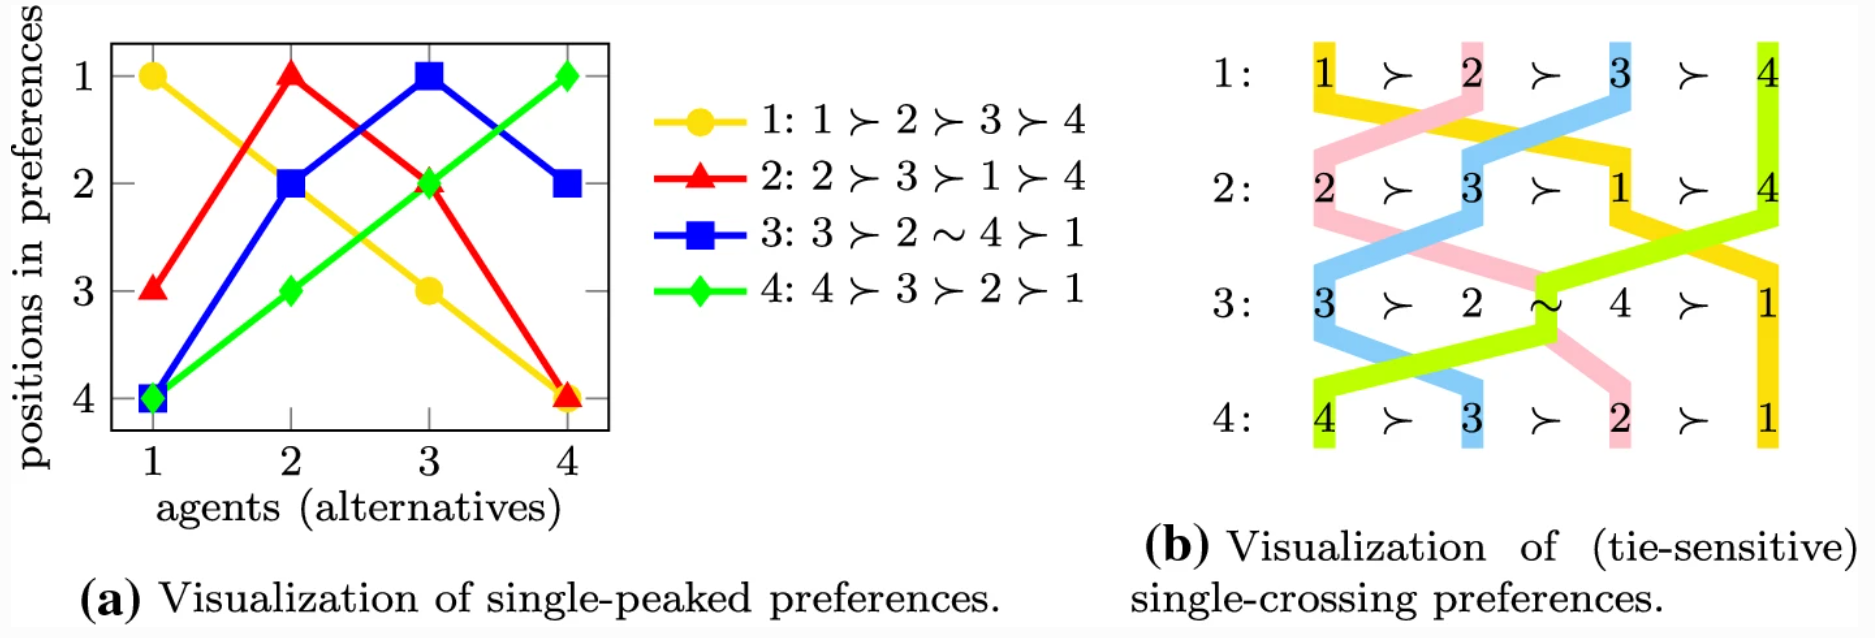
\includegraphics{../epol/fig/fig-02-005.png}

}

\caption{Pico único versus cruce único}

\end{figure}
\end{block}

\begin{block}{Aplicación: Modelo simple de redistribución}
\protect\hypertarget{aplicaciuxf3n-modelo-simple-de-redistribuciuxf3n}{}
\begin{itemize}
\tightlist
\item
  Hay \(\delta\) individuos ricos y \((1-\delta)\) individuos pobres con
  \(\delta < \frac{1}{2}\). Pobres tienen ingresos (exógenos) \(y^{p}\)
  y ricos \(y^{r}\)
\item
  Ingreso total \(\longrightarrow\) \(\delta y^{r}+(1-\delta)y^{p}=y\)
  --población normalizada a \(1\) por lo que \(y=\bar{y}\). Sea
  \(\theta\) fracción de \(y\) en manos de ricos tal que
  \(y^{r}=\frac{\theta y}{\delta}\) y que
  \(y^{p}=\frac{(1-\theta)y}{1-\delta}\)
\item
  Note que \(y^{r} > y^{p}\) y que \(\theta > \delta\). Aumento en
  \(\theta\) es más desigualdad, si \(\theta=\delta\), hay perfecta
  equidad \[\begin{aligned}
  c^{i}=(1-\tau)y^{i}+T \\
  T=\tau(\delta y^{r}+(1-\delta)y^{p})=\tau y
  \end{aligned}\]
\end{itemize}
\end{block}

\begin{block}{Aplicación: Modelo simple de redistribución (cont.)}
\protect\hypertarget{aplicaciuxf3n-modelo-simple-de-redistribuciuxf3n-cont.}{}
\begin{itemize}
\tightlist
\item
  Utilidad lineal en el consumo, \(u=c^{i}\). Sustituyendo RP del
  gobierno, la \(V\) es: \[\begin{aligned}
  V^{i}(\tau)=(1-\tau)y^{i}+\tau y
  \end{aligned}\]
\item
  Y la politica preferida maximiza \(V^{i}(\tau)\) por lo que:
  \[\begin{aligned}
  \frac{\partial V^{i}(\tau)}{\partial \tau}=-y^{i}+y
  \end{aligned}\]
\item
  Pobres \(\longrightarrow\) prefieren \(\tau=1\) (\(y\) menor al
  promedio); ricos \(\longrightarrow\) prefieren \(\tau=0\). Según el
  TVM \(\longrightarrow\) \(\tau^{eq}=1\) {[}¿Por qué?{]}
\end{itemize}
\end{block}

\begin{block}{Aplicación: Modelo simple de redistribución (cont.)}
\protect\hypertarget{aplicaciuxf3n-modelo-simple-de-redistribuciuxf3n-cont.-1}{}
\begin{itemize}
\tightlist
\item
  Mas realismo \(\longrightarrow\) hay costo asociado a la imposición
  (DWL) por lo que pobres no eligen \(\tau=1\). Ahora: \[\begin{aligned}
  T=\tau y - c(\tau)y
  \end{aligned}\]
\item
  donde \(c'(\tau)>0\), \(c''(\tau)>0\), \(c'(0)=0\), y
  \(c'(1)=\infty\). Con lo que la nueva \(V(.)\) es \[\begin{aligned}
  V^{i}(\tau)=(1-\tau)y^{i}+T=(1-\tau)y^{i} +\tau y - c(\tau)y
  \end{aligned}\]
\item
  CPO es \(c'(\tau^{eq})y=y-y^{i}\). De modo que ahora en \(\tau=1\),
  \(c'(\tau)=\infty\), y \emph{cualquier individuo} mejora utilidad con
  baja de T.
\end{itemize}
\end{block}

\begin{block}{Aplicación: Modelo simple de redistribución (cont.)}
\protect\hypertarget{aplicaciuxf3n-modelo-simple-de-redistribuciuxf3n-cont.-2}{}
\begin{itemize}
\tightlist
\item
  Para verificar preferencias unimodales, tomamos 2da derivada de V:
  \(-c''(\tau)<0\). Sustituyendo \(y^{p}=\frac{(1-\theta)y}{1-\delta}\)
  en CPO: \[\begin{aligned}
  c'(\tau^{p})=\frac{\theta-\delta}{1-\delta}
  \end{aligned}\]
\item
  Si \(\theta\) sube, \(\tau^{p}\) aumenta --interprete {[}Meltzer and
  Richard (1981){]}. Implicancias:

  \begin{itemize}
  \tightlist
  \item
    Mayor desigualdad, menor crecimiento {[}Persson and Tabellini
    (1994), Alesina and Rodrik (1994){]}
  \item
    ¿Por qué entonces los pobres votan? Los ricos tendrían incentivos a
    que no {[}Acemoglu and Robinson (2000){]}
  \end{itemize}
\end{itemize}
\end{block}
\end{frame}

\begin{frame}{\textbf{Reglas de votación}}
\protect\hypertarget{reglas-de-votaciuxf3n}{}
\begin{itemize}
\tightlist
\item
  Diferentes reglas de votación
\item
  Votación con ciclos: frecuencia y casos
\item
  Problemas y limitaciones del análisis
\item
  Intuición gráfica del TVM
\end{itemize}

\begin{block}{Votación Condorcet}
\protect\hypertarget{votaciuxf3n-condorcet}{}
\begin{itemize}
\tightlist
\item
  Suponga que un colectivo debe elegir entre 3 alternativas: A, B y C.
  Hay a priori 6 formas diferentes en que las preferencias pueden ser
  ordenadas:

  \begin{itemize}
  \tightlist
  \item
    \(A \succ_{1} B \succ_{1} C\)
  \item
    \(A \succ_{2} C \succ_{2} B\)
  \item
    \(B \succ_{3} A \succ_{3} C\)
  \item
    \(B \succ_{4} C \succ_{4} A\)
  \item
    \(C \succ_{5} A \succ_{5} B\)
  \item
    \(C \succ_{6} B \succ_{6} A\)
  \end{itemize}
\end{itemize}
\end{block}

\begin{block}{Votación Condorcet (cont.)}
\protect\hypertarget{votaciuxf3n-condorcet-cont.}{}
\begin{itemize}
\item
  \(A \succ_{1} B \succ_{1} C\)
\item
  \(B \succ_{4} C \succ_{4} A\)
\item
  \(C \succ_{6} B \succ_{6} A\)
\item
  Imagine ahora que se vota de a pares.

  \begin{itemize}
  \tightlist
  \item
    Voto entre A y B. ¿Quién gana? B
  \item
    Voto entre B y C. ¿Quién gana? B
  \item
    Voto entre C y A (¿es relevante?)
  \end{itemize}
\item
  ¿Hay alguna que gana a todas las demás? Si. La alternativa B. {[}¿Por
  qué A no puede ser un GdC? ¿Por qué C no es un GdC?{]}. La alternativa
  B es un \textbf{ganador de Condorcet}
\end{itemize}
\end{block}

\begin{block}{Votación Condorcet (cont.)}
\protect\hypertarget{votaciuxf3n-condorcet-cont.-1}{}
\begin{itemize}
\item
  \(A \succ_{1} B \succ_{1} C\)
\item
  \(B \succ_{4} C \succ_{4} A\)
\item
  \(C \succ_{5} A \succ_{5} B\)
\item
  Imagine ahora que se vota de a pares.

  \begin{itemize}
  \tightlist
  \item
    Voto entre A y B. ¿Quién gana? A
  \item
    Voto entre B y C. ¿Quién gana? B
  \item
    Voto entre C y A. ¿Quién gana? C
  \end{itemize}
\item
  ¿Cuál debería ganar si hay transitividad? A
\item
  No hay transitividad: \textbf{ciclo de Condorcet}
  \[A \succ B \succ C \succ A\]
\end{itemize}
\end{block}

\begin{block}{Ilustración: Fijar agenda}
\protect\hypertarget{ilustraciuxf3n-fijar-agenda}{}
\begin{itemize}
\tightlist
\item
  Supongamos que tenemos 30 personas cuyas preferencias por 4 (cuatro)
  alternativas se distribuyen de la siguiente manera:
\end{itemize}

\hypertarget{tab:tab1}{}
\begin{longtable}[]{@{}cc@{}}
\toprule()
votantes & preferencias \\
\midrule()
\endhead
10 & \(A \succ D \succ C \succ B\) \\
10 & \(B \succ A \succ D \succ C\) \\
10 & \(C \succ B \succ A \succ D\) \\
\bottomrule()
\end{longtable}

\begin{itemize}
\tightlist
\item
  ¿Puede \(D\) ganar democráticamente? Si, manipulando el orden de
  votación como la siguiente: 1) Voto entre \(B\) y \(A\); 2) Voto entre
  \(B\) y \(C\); 3) Voto entre \(C\) y \(D\) \(\longrightarrow\) todos
  disconformes con el resultado {[}¿Por qué?{]}
\end{itemize}
\end{block}

\begin{block}{Votación cíclica y agenda}
\protect\hypertarget{votaciuxf3n-cuxedclica-y-agenda}{}
\begin{itemize}
\tightlist
\item
  Recordando las preferencias que generaron un ciclo de Condorcet. Sea
  el orden de votación::

  \begin{itemize}
  \tightlist
  \item
    1ra: A vs B. 2da: ganador de A vs B contra C

    \begin{itemize}
    \tightlist
    \item
      Dado que \(A \succ B\) y \(C \succ A\), \uline{gana C}
    \end{itemize}
  \item
    1ra: A vs C. 2da: ganador de A vs C contra B

    \begin{itemize}
    \tightlist
    \item
      Dado que \(C \succ A\) y \(B \succ C\), \uline{gana B}
    \end{itemize}
  \item
    1ra: B vs C. 2da: ganador de B vs C contra A

    \begin{itemize}
    \tightlist
    \item
      Dado que \(B \succ C\) y \(A \succ B\), \uline{gana A}.
    \end{itemize}
  \end{itemize}
\item
  El ganador depende depende del orden de votación! \(\longrightarrow\)
  problema de los ciclos
\end{itemize}
\end{block}

\begin{block}{Ciclos con alternativas no definidas}
\protect\hypertarget{ciclos-con-alternativas-no-definidas}{}
\begin{itemize}
\tightlist
\item
  Suponga que tres legisladores deben elegir como distribuir un
  presupuesto de 1000 pesos entre tres provincias

  \begin{itemize}
  \tightlist
  \item
    Inicial \(\longrightarrow\) \((333.3,333.3,333.3)\)
  \item
    Propuesta de 1 \(\longrightarrow\) \((600,400,0)\) {[}gana por
    mayoría{]}
  \item
    Propuesta de 3 \(\longrightarrow\) \((0,600,400)\) {[}gana por
    mayoría{]}
  \item
    Propuesta de 1 \(\longrightarrow\) \((300,700,0)\) {[}gana por
    mayoría{]}
  \item
    Propuesta de 3 \(\longrightarrow\) \((333.3,333.3,333.3)\) y
    así\ldots{}
  \end{itemize}
\item
  Este problema es conocido como el de \textbf{dividir un dólar} y
  muestra como existen ciclos \(\longrightarrow\) alternativas no
  definidas
\end{itemize}
\end{block}

\begin{block}{Ciclos con alternativas definidas}
\protect\hypertarget{ciclos-con-alternativas-definidas}{}
\begin{itemize}
\tightlist
\item
  Sea un problema redistributivo similar pero con alternativas fijas,
  \(x\), \(y\), \(z\). Eje vertical, cantidad de recursos de B; eje
  horizontal, cantidad de recursos de A, y el resto es para C. Líneas
  son las CI de cada político. Votación:

  \begin{itemize}
  \tightlist
  \item
    \(y\) contra \(z\), gana \(y\)
  \item
    \(y\) contra \(x\), gana \(x\)
  \item
    \(x\) contra \(z\), gana \(z\)
  \end{itemize}
\item
  Posible ciclo infinito aún con nro limitado de alternativas
  --respetando supuestos básicos
\end{itemize}
\end{block}

\begin{block}{Ciclos con alternativas definidas (cont.)}
\protect\hypertarget{ciclos-con-alternativas-definidas-cont.}{}
\begin{figure}

{\centering 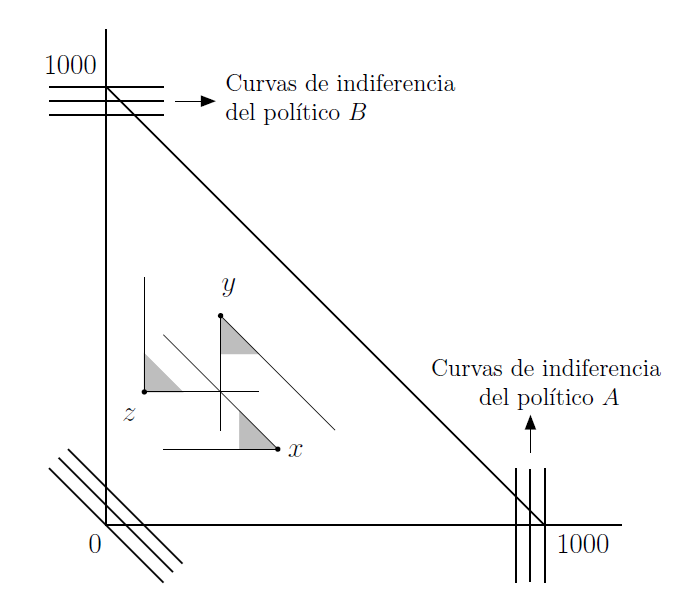
\includegraphics[width=0.7\textwidth,height=\textheight]{../epol/fig/fig-02-014.png}

}

\caption{Ciclos e indeterminaciones}

\end{figure}
\end{block}

\begin{block}{Ocurrencia de ciclos}
\protect\hypertarget{ocurrencia-de-ciclos}{}
\begin{figure}

{\centering 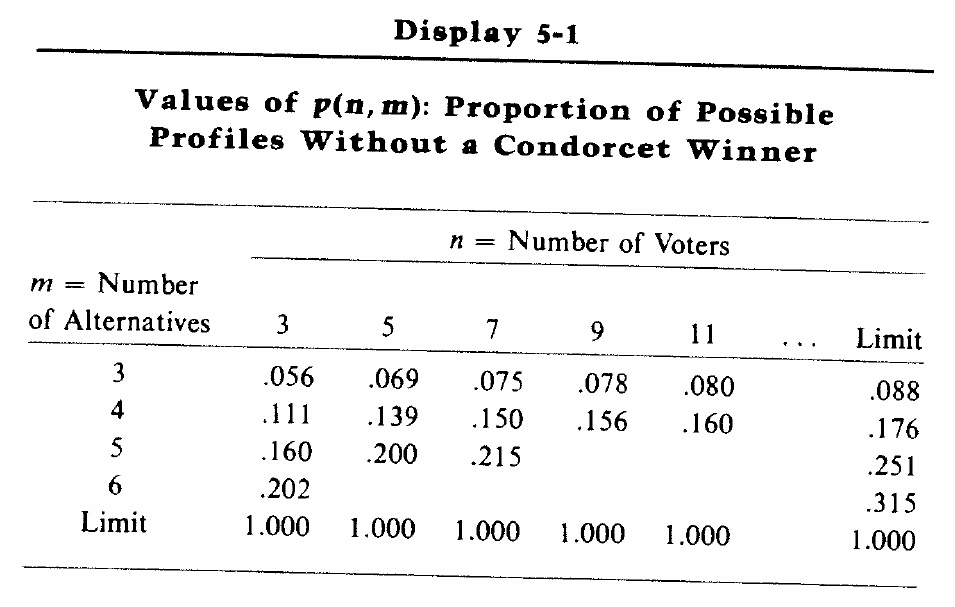
\includegraphics[width=0.8\textwidth,height=\textheight]{../epol/fig/fig-02-015.png}

}

\caption{Perfiles de preferencias sin ganador de Condorcet}

\end{figure}
\end{block}

\begin{block}{Limitando ciclos: agenda cerrada}
\protect\hypertarget{limitando-ciclos-agenda-cerrada}{}
\begin{itemize}
\tightlist
\item
  Una forma es limitar número de rondas. Garantiza una política pero no
  sabemos cuál! Manipular agenda \(\longrightarrow\) otorga poder a
  quien la controla ya que puede elegir su política preferida
  (\emph{votación sincera}). Pero hay incentivos a votar
  estratégicamente

  \begin{itemize}
  \tightlist
  \item
    \(B\) vota por \(z\) en ronda 1 y obtiene \(y\) en ronda 2
    pero\ldots{}
  \item
    \(A\) y \(C\) también querrán ser estrategicos

    \begin{itemize}
    \tightlist
    \item
      equilibrios múltiples surgen facilmente
    \end{itemize}
  \end{itemize}
\item
  ¿Votación sincera realista?

  \begin{itemize}
  \tightlist
  \item
    Si, cuando hay 2 alternativas
  \item
    Si, cuando hay muchos votantes y ninguno es decisivo
  \end{itemize}
\end{itemize}
\end{block}

\begin{block}{Poder de agenda}
\protect\hypertarget{poder-de-agenda}{}
\begin{itemize}
\tightlist
\item
  Este simple ejemplo ilustra la importancia del ``poder de agenda''
  --qué alternativas considerar y en qué orden las votamos.
\item
  ¿Quiénes establecen la agenda en la vida real?

  \begin{itemize}
  \tightlist
  \item
    En el Congreso, el Presidente de la Cámara y los Presidentes de
    Comisión tienen amplios poderes para decidir que asuntos se giran y
    para proponer el orden de votaciones en el recinto. En EEUU, es el
    Speaker of the House
  \item
    En regímenes presidencialistas, los ejecutivos también tienen poder
    de agenda (DNU, vetos, poderes delegados)
  \end{itemize}
\item
  El poder de agenda no es ilimitado ni da control absoluto, pero da
  alguna ventaja
\end{itemize}
\end{block}

\begin{block}{Votación Borda}
\protect\hypertarget{votaciuxf3n-borda}{}
\begin{itemize}
\tightlist
\item
  El \textbf{método de Borda} es una alternativa a Condorcet para
  superar el problema de los ciclos. Sean 5 votantes y 3 alternativas
  tal que:
\end{itemize}

\hypertarget{tab:tab2}{}
\begin{longtable}[]{@{}cccccc@{}}
\toprule()
Orden & 1 & 2 & 3 & 4 & 5 \\
\midrule()
\endhead
1 & A & A & A & B & B \\
2 & B & B & B & C & C \\
3 & C & C & C & A & A \\
\bottomrule()
\end{longtable}

\begin{itemize}
\tightlist
\item
  Cada individuo (grupo de individuos) van a puntuar las alternativas
  según el lugar (orden) que ocupen en el ordenamiento. A diferencia de
  Condorcet, este método usa toda la información de preferencias
  (intensidad de las preferencias).
\end{itemize}
\end{block}

\begin{block}{Votación Borda (cont.)}
\protect\hypertarget{votaciuxf3n-borda-cont.}{}
\begin{itemize}
\tightlist
\item
  Existen dos implementaciones alternativas del método de Borda:

  \begin{itemize}
  \tightlist
  \item
    La alternativa en 1er lugar recibe \(n\) puntos, la alternativa en
    2do lugar, recibe \(n-1\) puntos, y así hasta la última alternativa
    donde ``n'' es el número de alternativas.
  \item
    La alternativa en primer lugar recibe \(n-1\) puntos, la alternativa
    en segundo lugar, recibe \(n-2\) puntos, y así hasta la última donde
    ``n'' es el número de alternativas.
  \item
    Pueden utilizarse ambos criterios a menos que esté explícitamente
    indicado un criterio en el ejercicio y/o práctico.
  \end{itemize}
\end{itemize}
\end{block}

\begin{block}{Votación Borda (cont.)}
\protect\hypertarget{votaciuxf3n-borda-cont.-1}{}
\begin{itemize}
\tightlist
\item
  En este caso (solucionando por método ``n-1'', las alternativas
  recibirían:

  \begin{itemize}
  \tightlist
  \item
    \(A\) \(\longrightarrow\) 6 votos
  \item
    \(B\) \(\longrightarrow\) 7 votos
  \item
    \(C\) \(\longrightarrow\) 2 votos
  \end{itemize}
\item
  Parece un método razonable aunque algo difícil de implementar
  \(\longrightarrow\) el candidato C podría desistir de presentarse. En
  ese caso, la primera alternativa recibe 1 (uno) y la segunda 0 (cero).
\end{itemize}
\end{block}

\begin{block}{Votación Borda (cont.)}
\protect\hypertarget{votaciuxf3n-borda-cont.-2}{}
\begin{itemize}
\tightlist
\item
  Ahora con este nuevo esquema, el ganador es \(A\)! (obtiene 3 contra 2
  votos de \(B\)) \(\longrightarrow\) presencia o no de alternativas
  irrelevantes --\(C\)- puede modificar el resultado de la elección
\item
  Este método sin embargo se usa mucho en eventos y competiciones
  musicales y en elección de sedes, mejores jugadores, etc.
\item
  El principal problema del método Borda \(\longrightarrow\) viola el
  principio de mayoría y viola el ganador de Condorcet
\end{itemize}
\end{block}

\begin{block}{El rol del mediano}
\protect\hypertarget{el-rol-del-mediano}{}
\begin{figure}

{\centering 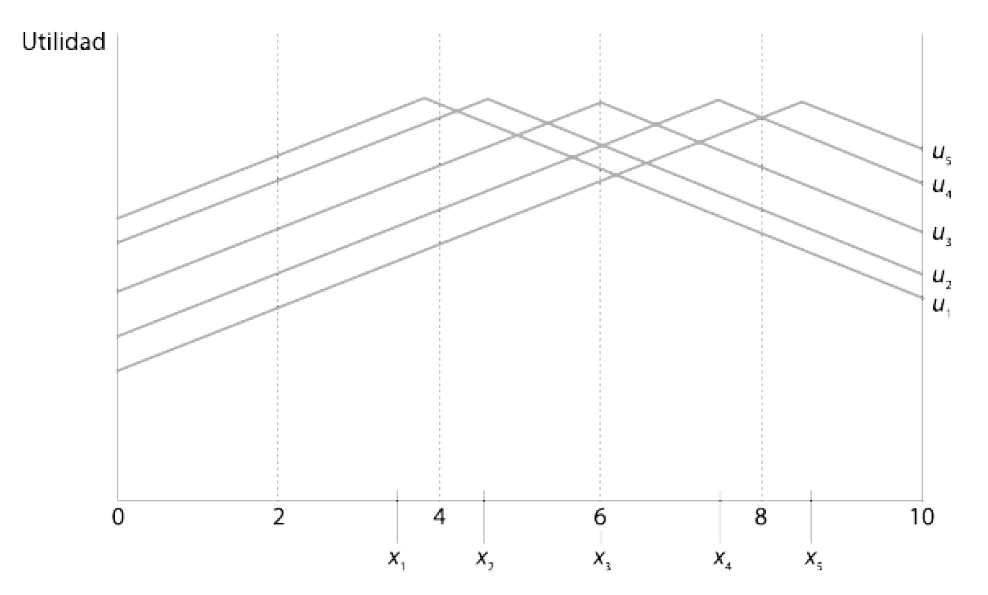
\includegraphics{../epol/fig/fig-02-006.png}

}

\caption{Preferencias a lo largo de una linea}

\end{figure}
\end{block}

\begin{block}{El rol del mediano (cont.)}
\protect\hypertarget{el-rol-del-mediano-cont.}{}
\begin{itemize}
\tightlist
\item
  Las cinco personas, \(G={1,2,3,4,5}\) tienen las preferencias
  mostradas en el gráfico anterior y representadas como
  \(x={x_1,x_2,x_3,x_4,x_5}\).
\item
  Cada individuo tiene un punto favorito \(\longrightarrow\) ``punto
  ideal''. Esa es la tasa de interés que el/ella prefiere en primer
  lugar. Por ejemplo, para el director 1:

  \begin{itemize}
  \tightlist
  \item
    \(x_1 \succ x_2 \succ x_3 \succ x_4 \succ x_5\)
  \end{itemize}
\item
  Las preferencias se ``miden'' a partir de la utilidad --i.e.~la altura
  de la curva; cada una de las ``campanas'' es una función de utilidad
  para cada director.
\end{itemize}
\end{block}

\begin{block}{El rol del mediano (cont.)}
\protect\hypertarget{el-rol-del-mediano-cont.-1}{}
\begin{figure}

{\centering 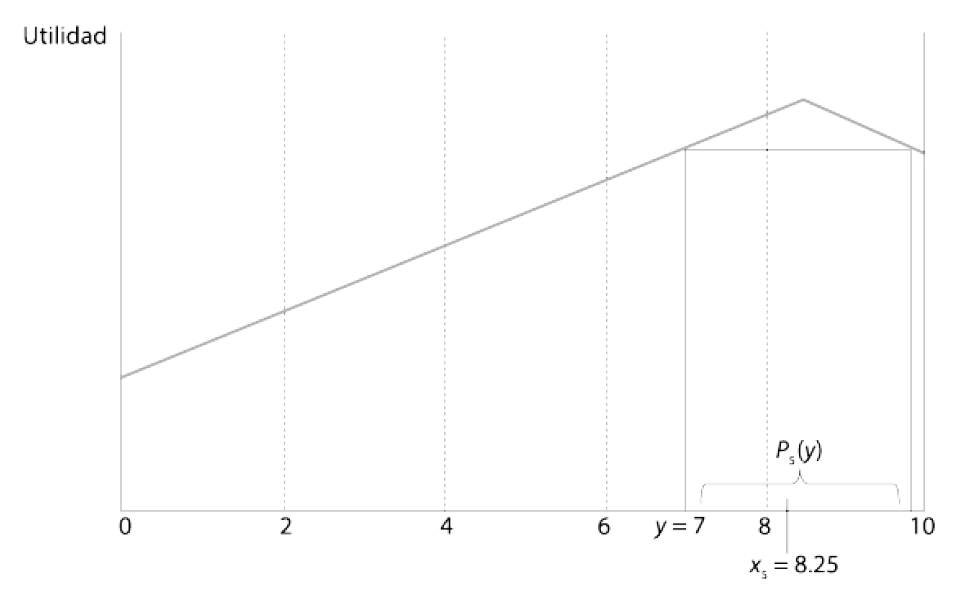
\includegraphics[width=0.9\textwidth,height=\textheight]{../epol/fig/fig-02-007.png}

}

\caption{Conjuntos preferidos}

\end{figure}
\end{block}

\begin{block}{El rol del mediano (cont.)}
\protect\hypertarget{el-rol-del-mediano-cont.-2}{}
\begin{itemize}
\tightlist
\item
  Tomemos ahora solamente al individuo 5. Su perfil de preferencias es
  \(x_5 \succ x_4 \succ x_3 \succ x_2 \succ x_1\). Su tasa de interés
  favorita (punto ideal) es de \(8.25\).
\item
  Tomemos una tasa cualquiera --i.e.~\(7\). El conjunto de puntos
  (tasas) que este individuo prefiere a \(7\) es el que se representa
  como \(P_5(y)\): ese conjunto contiene a todas las tasas de interés
  entre 7 y 9.25 {[}¿Por qué?{]}
\item
  En otras palabras, si la tasa \(y\) fuera una propuesta concreta, este
  individuo prefería todos los puntos del conjunto \(P_5(y)\) a \(y\).
\end{itemize}
\end{block}

\begin{block}{El rol del mediano (cont.)}
\protect\hypertarget{el-rol-del-mediano-cont.-3}{}
\begin{figure}

{\centering 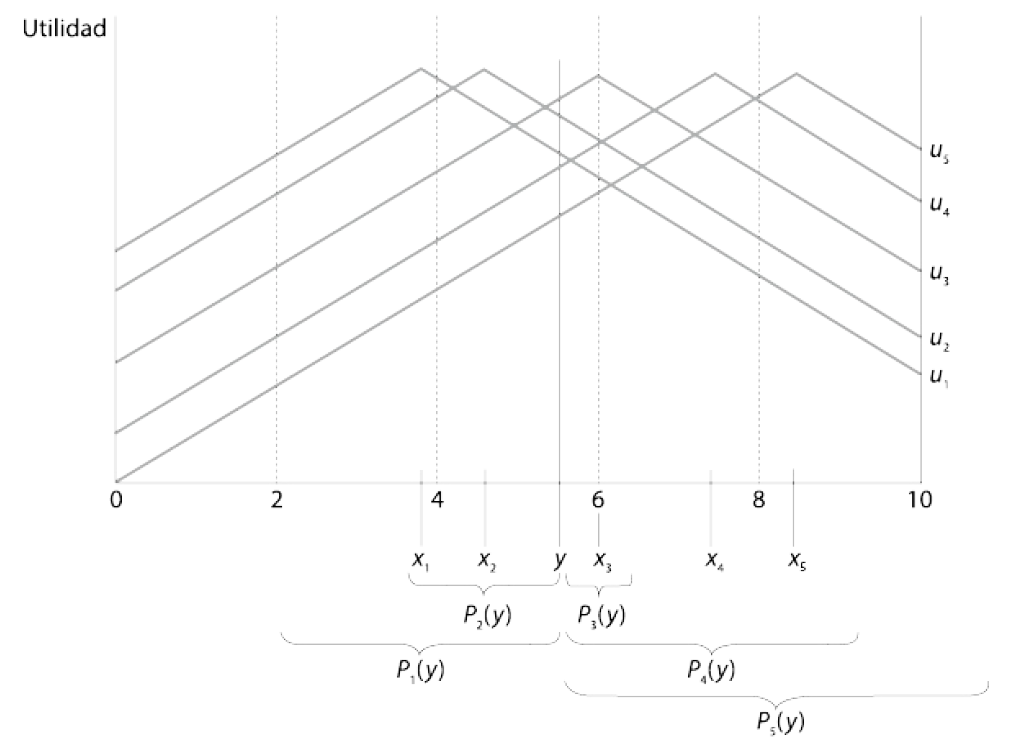
\includegraphics[width=0.8\textwidth,height=\textheight]{../epol/fig/fig-02-008.png}

}

\caption{Superponiendo los conjuntos preferidos}

\end{figure}
\end{block}

\begin{block}{El rol del mediano (cont.)}
\protect\hypertarget{el-rol-del-mediano-cont.-4}{}
\begin{itemize}
\tightlist
\item
  Ahora mostramos los ``conjuntos preferidos a \(y\)'' de todos los
  directores.Superposición:

  \begin{itemize}
  \tightlist
  \item
    \(P_4(y)\) y \(P_5(y)\) tienen puntos en común
  \item
    \(P_1(y)\) y \(P_2(y)\) tienen puntos en común
  \item
    Los individuos 3, 4 y 5 tienen conjuntos preferidos a \(y\) que se
    superponen; forman una mayoría --3 contra 2, por lo que esa mayoría
    vence a una propuesta como \(y\).
  \end{itemize}
\item
  Así, se tienen todas las mayorías posibles que vencen a \(y\)
  dependiendo de donde este \(y\) en la escala.Puede ahora mostrarse
  todas las coaliciones de mayorías posibles que vencen a \(y\).
\end{itemize}
\end{block}

\begin{block}{El rol del mediano (cont.)}
\protect\hypertarget{el-rol-del-mediano-cont.-5}{}
\hypertarget{tab:1}{}
\begin{longtable}[]{@{}cl@{}}
\toprule()
Tamaño coalicion & Coalicion \\
\midrule()
\endhead
3 & (1,2,3) (1,2,4) (1,2,5) (1,3,4) (1,3,5) (1,4,5) (2,3,4) (2,3,5)
(2,4,5) (3,4,5) \\
4 & (1,2,3,4) (1,2,3,5) (1,2,4,5) (1,3,4,5) (2,3,4,5) \\
5 & (1,2,3,4,5) \\
\bottomrule()
\end{longtable}
\end{block}

\begin{block}{El rol del mediano (cont.)}
\protect\hypertarget{el-rol-del-mediano-cont.-6}{}
\begin{figure}

{\centering 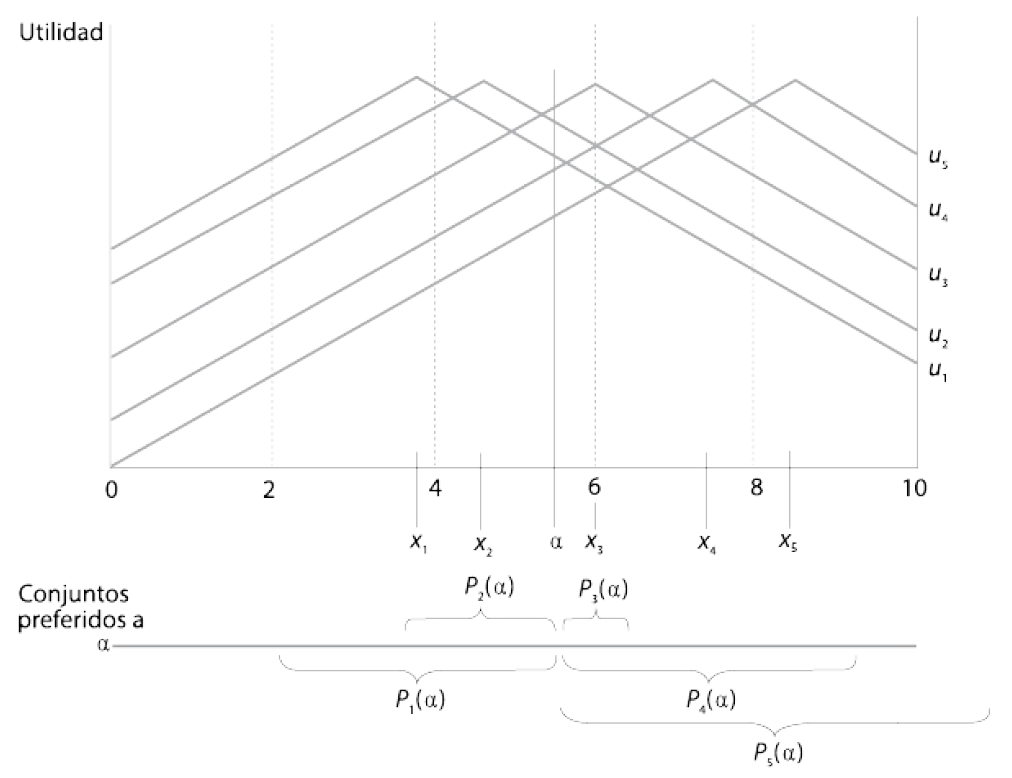
\includegraphics[width=0.8\textwidth,height=\textheight]{../epol/fig/fig-02-009.png}

}

\caption{El rol del votante mediano}

\end{figure}
\end{block}
\end{frame}



\end{document}
